\subsection{Sequence Diagram}

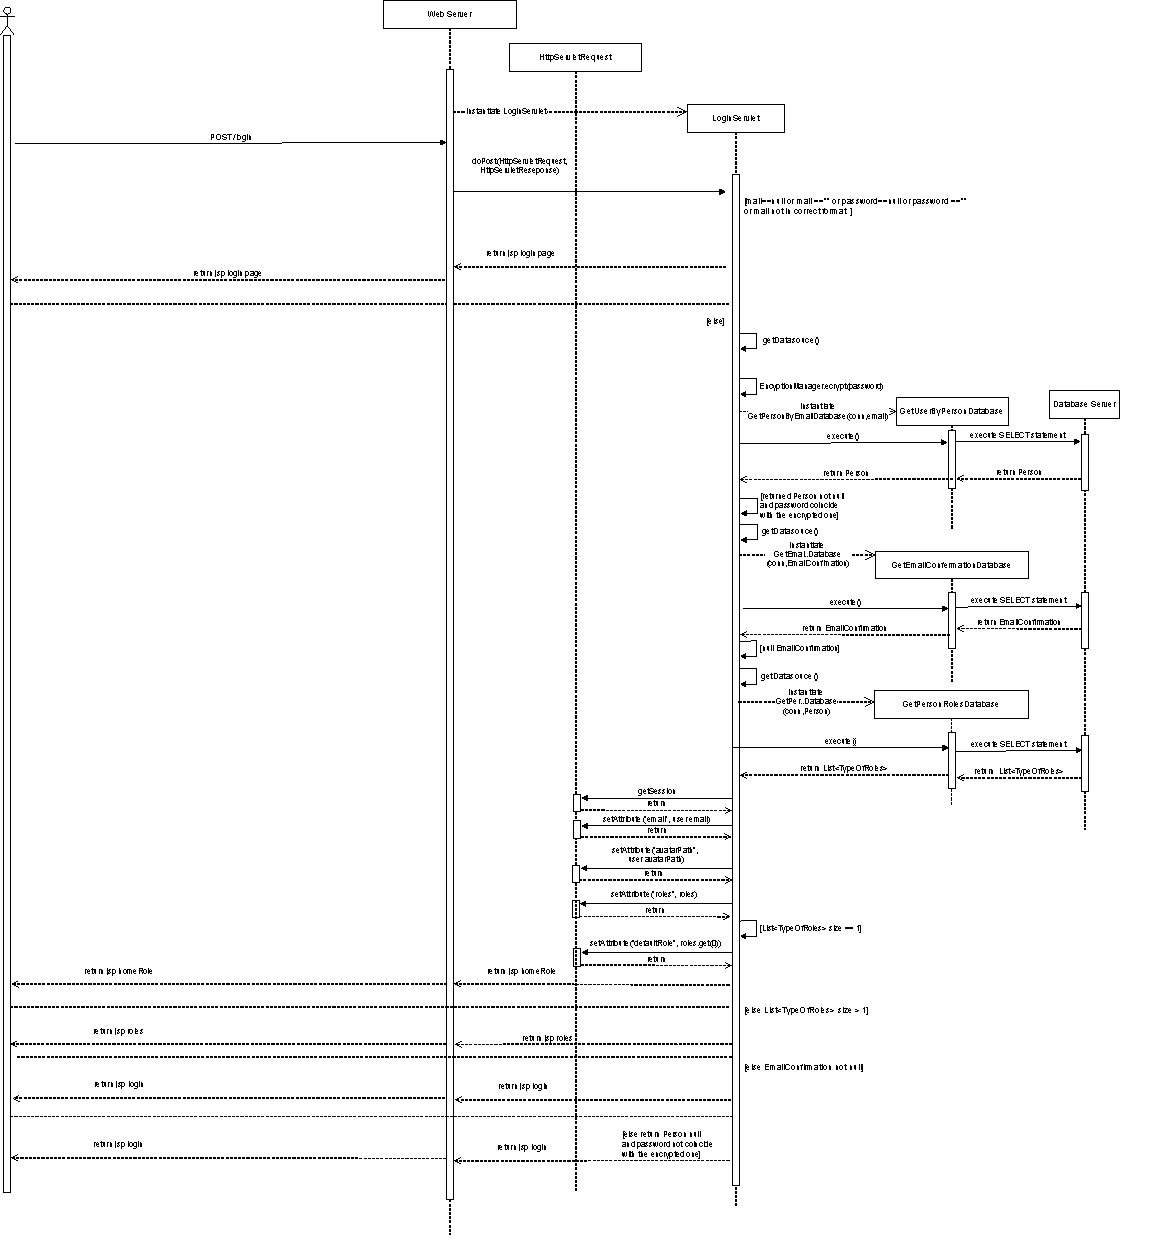
\includegraphics[width=\columnwidth,height=\textheight]{resources/Sequence_Diagram2-cropped.pdf}

\begin{flushleft}
Here reported the sequence diagram for the login operations. 

The user executes a POST request to the web server, specifying the URI /login. Additionally, the data about the user which is trying to login (email and password) are passed to the web server. The web server instantiates the LoginServlet and calls its doPost method, passing the HttpServletRequest and the HttpServlet response. The LoginServlet analyzes the request and test if the mail and password are both  null or equal to the empty string. If so, then it is returned the login jsp page with an error. Otherwise it is called the getDataSource method and the EcyptionManager.encrypt() method (the latter) to encrypt the password. Moreover, a DAO called GetPersonByEmailDatabase is intialized using a connection and the email. Then, it is called the execute() method of the DAO and if everything is fine a Person is returned. Addtionaly it is tested if the user returned is not null and his password coincide with the encrypted one, if so, a new DAO called GetEmailConfirmationDatabase is istantiated and the execute() method of the DAO is called. Furthermore, it is tested if the EmailConfirmation object returned is not null, and finally it is istantiated the last DAO called GetPersonRolesDatabase and called his method execute().
Therefore now it is obtained the session through the method getSession and set as attributes : email, avatarpath, defaultRole and list of roles of the User.
Finally the following pages are returned :
\begin{itemize}
	\item homeRole if the listofroles has size 1
	\item roles if the listofroles has size grater than 1
	\item the login page with an error if the emailconfirmation object returned by the GetEmailConfirmationDatabase was not null (becasue the user has not completed the registration) 
	\item the login page with an error if the either the person was null or the password did not coincide with the encrypted one for such Person from the GetUserByEmailDatabase DAO
\end{itemize}

\end{flushleft}



%describe here the sequence diagram